% --------------------------------------------------------------
% This is all preamble stuff that you don't have to worry about.
% Head down to where it says "Start here"
% --------------------------------------------------------------
 
\documentclass[12pt]{article}
\usepackage[margin=1in]{geometry} 
\usepackage{amsmath,amsthm,amssymb}
\usepackage[margin=1in]{geometry} 
\usepackage{amsmath,amsthm,amssymb}
\usepackage[utf8]{inputenc}
\usepackage[T1]{fontenc} %escribe lo del teclado
\usepackage[utf8]{inputenc} %Reconoce algunos símbolos
\usepackage{lmodern} %optimiza algunas fuentes
\usepackage{graphicx}
\graphicspath{ {images/} }
\usepackage{hyperref} % Uso de links
\usepackage{float}
\usepackage{subfig}
\usepackage{tabto}
\usepackage{amsmath}
\hypersetup{
    colorlinks=true,
    linkcolor=blue,
    filecolor=magenta,      
    urlcolor=cyan,
}
\date{}


\newcommand{\N}{\mathbb{N}}
\newcommand{\Z}{\mathbb{Z}}
 
\newenvironment{theorem}[2][Theorem]{\begin{trivlist}
\item[\hskip \labelsep {\bfseries #1}\hskip \labelsep {\bfseries #2.}]}{\end{trivlist}}
\newenvironment{lemma}[2][Lemma]{\begin{trivlist}
\item[\hskip \labelsep {\bfseries #1}\hskip \labelsep {\bfseries #2.}]}{\end{trivlist}}
\newenvironment{exercise}[2][Exercise]{\begin{trivlist}
\item[\hskip \labelsep {\bfseries #1}\hskip \labelsep {\bfseries #2.}]}{\end{trivlist}}
\newenvironment{problem}[2][Problem]{\begin{trivlist}
\item[\hskip \labelsep {\bfseries #1}\hskip \labelsep {\bfseries #2.}]}{\end{trivlist}}
\newenvironment{question}[2][Question]{\begin{trivlist}
\item[\hskip \labelsep {\bfseries #1}\hskip \labelsep {\bfseries #2.}]}{\end{trivlist}}
\newenvironment{corollary}[2][Corollary]{\begin{trivlist}
\item[\hskip \labelsep {\bfseries #1}\hskip \labelsep {\bfseries #2.}]}{\end{trivlist}}

\newenvironment{solution}{\begin{proof}[Solution]}{\end{proof}}
 
\begin{document}

% --------------------------------------------------------------
%                         Start here
% --------------------------------------------------------------
 
\title{Práctica 3: Detección de puntos relevantes y Construcción de panoramas}
\author{Víctor Manuel Arroyo Martín\\ %replace with your name
Visión por Computador}

\maketitle
\section*{Introducción}
El código lo he escructurado en una sección de funciones auxiliares, otra sección con las funciones necesarias para cada apartado y una parte final donde se ejecutan e imprimen esas funciones para solucionar la práctica.\\
Los puntos de parada los he incluido de forma que separen apartados y ejercicios, así que es posible que se muestran varias imágenes seguidas si son del mismo apartado o ejercicio.\\
\section*{Ejercicio 1: Detección de puntos Harris}
En este ejercicio se pide usar el detector de Harris para detectar esquinas en las imágenes. Los resultados los mostraré sobre las dos imágenes de Yosemite que se nos ha proporcionado.\\
\subsection*{Apartado a) Pirámide Gaussiana}
Primero creamos una pirámide gaussiana de la imagen con la función \texttt{gaussianPyramid} que hace uso de \texttt{pyrDown} de OpenCV para crear la lista de imágenes de la pirámide.\\
\begin{figure}[H]
\centering
\includegraphics[scale=0.35]{images/pirGaussYosemite1.png} 
\caption{Pirámide Gaussiana para Yosemite1.}
\label{etiqueta}
\end{figure}
\begin{figure}[H]
\centering
\includegraphics[scale=0.35]{images/pirGaussYosemite2.png} 
\caption{Pirámide Gaussiana para Yosemite2.}
\label{etiqueta}
\end{figure}
Después en la función \texttt{harrisDetection}, con un tamaño de block-size de 3x3 y un ksize de 3, usamos la función \texttt{cornerEigenValsAndVecs} para extraer de cada punto p información sobre la matriz de covarianzas de las derivadas en un entorno S(p). La matriz la calcula como:\\
\begin{equation}
\begin{pmatrix}
\sum_{S(p)}(dI/dx)^{2} & \sum_{S(p)}dI/dx dI/dy\\
\sum_{S(p)}dI/dx dI/dy & \sum_{S(p)}(dI/dy)^{2} \\
\end{pmatrix}
\end{equation} 
Esta función nos devuelve una matriz con 6 canales y nos quedamos con los dos primeros que es donde se encuentran los valores propios $\lambda_{1}(p)$ y $\lambda_{2}(p)$.\\
El parámetro blockSize determina el tamaño del vecindario S(p) antes nombrado, siendo un 3x3 como recomienda el enunciado. El tercer parámetro indica el tamaño de los kernels para calcular derivadas, también lo he puesto a 3 como se pide en el enunciado.\\
Tras ello, calculamos el operador de Harris, que es la matriz de valores para el criterio de Harris, siguiendo las diapositivas de teoría:\\
\begin{equation}
f=\frac{\lambda_{1} \lambda_{2}}{\lambda_{1}+\lambda_{2}}
\end{equation}
Que es la media armónica de los valores propios asociados. Esta función mide la intensidad de las direcciones propias de la matriz anterior con lo que si f da un valor alto, quiere decir que hay dos direcciones intensas en un punto y por tanto hay una esquina. La matriz f representada en una imagen queda como sigue para cada nivel de la pirámide gaussiana:\\
Para Yosemite1:\\
\begin{figure}[H]
\centering
\parbox{8cm}{
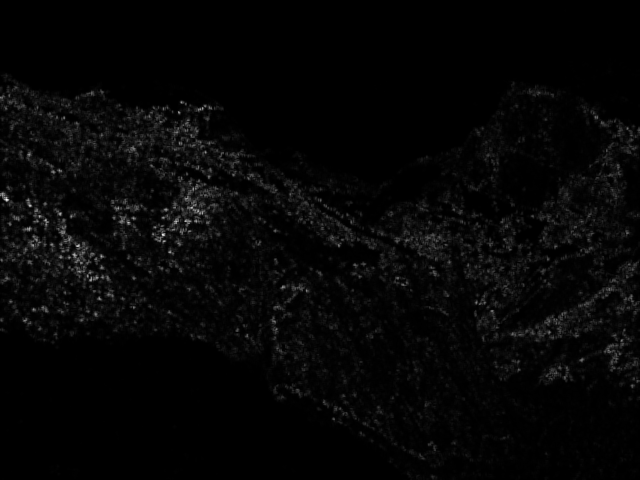
\includegraphics[width=6cm]{images/fYosemite1-0.png}
\caption{Nivel 0}
\label{fig:3figsA}}
\begin{minipage}{5cm}
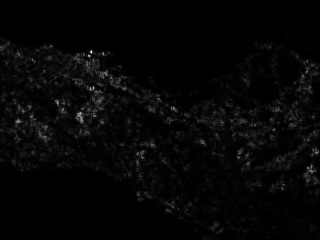
\includegraphics[width=4cm]{images/fYosemite1-1.png}
\caption{Nivel 1}
\label{fig:3figsB}
\end{minipage}
\begin{minipage}{3cm}
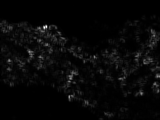
\includegraphics[width=3cm]{images/fYosemite1-2.png}
\caption{Nivel 2}
\label{fig:3figsC}
\end{minipage}
\end{figure}
Para Yosemite2:\\
\begin{figure}[H]
\centering
\parbox{8cm}{
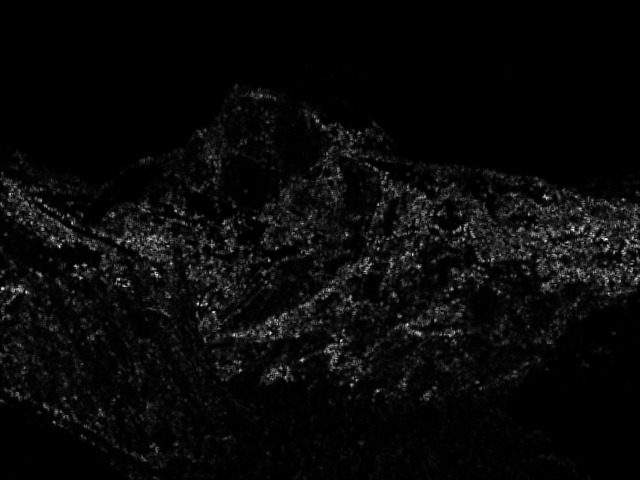
\includegraphics[width=6cm]{images/fYosemite2-0.png}
\caption{Nivel 0}
\label{fig:3figsA}}
\begin{minipage}{5cm}
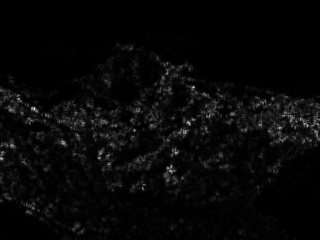
\includegraphics[width=4cm]{images/fYosemite2-1.png}
\caption{Nivel 1}
\label{fig:3figsB}
\end{minipage}
\begin{minipage}{3cm}
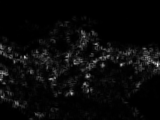
\includegraphics[width=3cm]{images/fYosemite2-2.png}
\caption{Nivel 2}
\label{fig:3figsC}
\end{minipage}
\end{figure}

\subsection*{Apartado b) Supresión de no-máximos}
Para la supresión de no-máximos he creado una función llamada \texttt{nonMaxiumSupression} donde nos quedamos sólo con los puntos que superan cierto umbral y que son máximos locales en un entorno de 7x7 para la escala más grande y 3x3 para la más pequeña en la pirámide.\\
En la función \texttt{harrisDetection}, las siguientes líneas calculan la supresión de no máximos:
\begin{center}
\texttt{indice$\_$max = nonMaxiumSupression(f, window)}\\
\texttt{indice$\_$max = sorted(indice$\_$max, key = lambda x: f[x], reverse = True)}
\end{center}
En cada nivel nos vamos a quedar con un número fijo de puntos, con las proporciones (70$\%$-25$\%$-5$\%$) de 2000 puntos: [1500, 400, 100] por cada nivel.

\subsection*{Apartado c) Escala y orientación de KeyPoints}
Con cada punto que queda de la supresión, calculamos la estructura KeyPoints donde guardamos la columna y la fila (en ese orden), el tamaño y el ángulo. Para ello alisamos y calculamos las derivadas en x e y y alisamos la imagen como se pide en el enunciado, con un sigma de 4.5:\\
\begin{center}
\texttt{img$\_$G = cv2.GaussianBlur(im, ksize = (0, 0), sigmaX = 4.5)}\\
\texttt{img$\_$dx = gaussianPyramid(cv2.Sobel(img$\_$G, -1, 1, 0), 2)}\\
\texttt{img$\_$dy = gaussianPyramid(cv2.Sobel(img$\_$G, -1, 0, 1), 2)}\\
\end{center}
Para calcular el ángulo o la orientación de cada punto consideramos el vector unitario (cos$\theta$, sin$\theta$) = u/|u|, donde u proviene del gradiente (local) alisado: u = $\bigtriangledown_{\sigma}$ I, con $\sigma$ = 4.5.\\
\subsection*{Apartado d) Mostrar los resultados de los KeyPoints}
Tras calcular el ángulo, guardamos los key points con sus escalas como se indica en el enunciado y tras acabar los del nivel correspondiente, los dibujamos con la función \texttt{drawKeypoints} de OpenCV en la imagen del nivel correspondiente.\\
Como se puede ver por pantalla, se obtienen los puntos que se indicaban al principio: [1500, 400, 100] para cada nivel. Las imágenes para las pirámides de yosemite 1 y 2 con los puntos dibujados quedan:
\begin{figure}[H]
\centering
\parbox{8cm}{
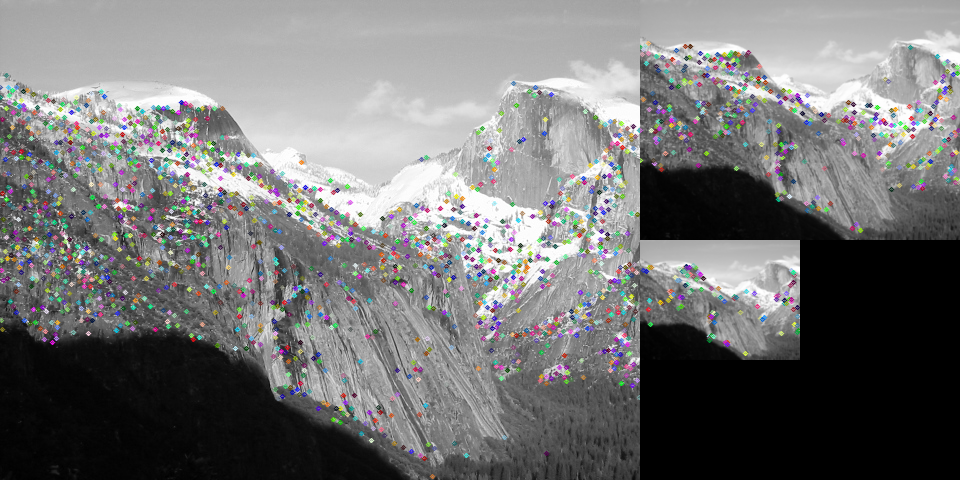
\includegraphics[width=8cm]{images/PirHarrisYosemite1.png}
\caption{Pirámide para yosemite1}
\label{fig:2figsA}}
\begin{minipage}{8cm}
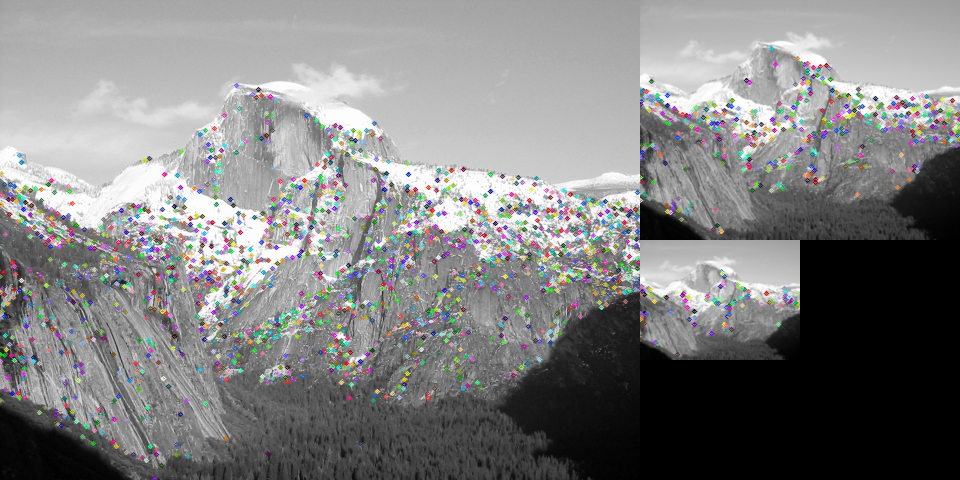
\includegraphics[width=8cm]{images/PirHarrisYosemite2.png}
\caption{Pirámide para yosemite2}
\label{fig:2figsB}
\end{minipage}
\end{figure}
Vemos que son un conjunto representativo de puntos para cada escala pues los puntos están repartidos por toda la imagen y no concentrados en una sola parte. El número de puntos es suficiente y más puntos saturaría la imagen impidiendo ver las esquinas más relevantes.

\subsection*{Apartado e) Refinamiento}
Ahora refinamos los puntos obtenidos con precisión decimal (a nivel subpixel). Para ello, usamos la función \texttt{cornerSubPix} de OpenCv a la que le pasamos una lista con las coordenadas detectadas y un tamaño de ventana. La función se encarga de refinar las coordenadas de las esquinas en un entorno definido por dos veces el tamaño proporcionado, hasta cumplir un cierto criterio de parada, en este caso he elegido de parada hasta 100 iteraciones o que las coordenadas difieran más de 0.01 en una iteración.\\
Hacemos un doble refinamiento con esta función:
\begin{center}
\texttt{cv2.cornerSubPix(im, esquinas, win$\_$size, zero$\_$zone, criteria)}\\
$\#$Para las dos capas superiores volvemos a hacer un refinamiento con venatana 5x5\\
\texttt{esquinas2 = esquinas[-1400:]}
\texttt{cv2.cornerSubPix(im, esquinas2, win$\_$size2, zero$\_$zone, criteria)}
\end{center}
El primer refinamiento es con un tamaño de ventana de 7x7 y el segundo con uno de 5x5 como se indica en el enunciado. El parámetro \texttt{zero$\_$zone} se usa para indicar que no se debe ignorar ninguna región de búsqueda.\\
Para mostrar los resultados, seleccionamos una región con un zoom de 7x (lo he cambiado de lo que dice el enunciado porque con 10x al estar tan cerca muchas veces no salen los puntos corregidos en la imagen). Quedan las siguientes imágenes:\\
\begin{figure}[H]
\centering
\parbox{8cm}{
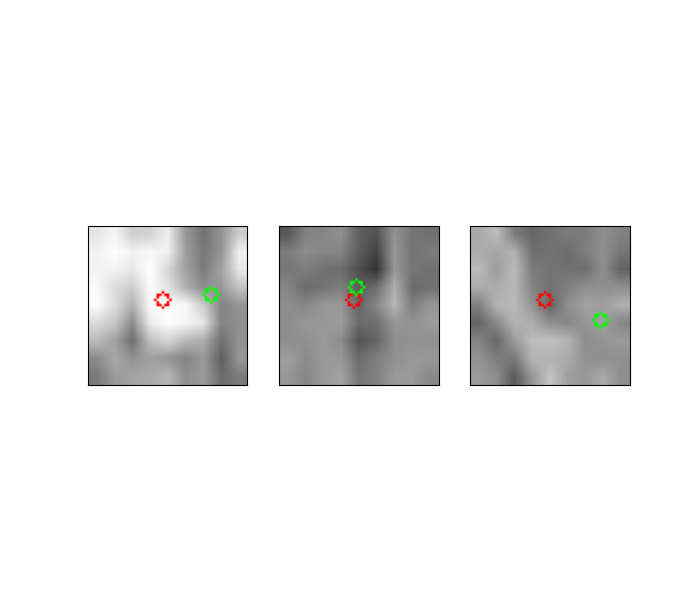
\includegraphics[width=9cm]{images/Refinado1.png}
\caption{Puntos refinados para yosemite1}
\label{fig:2figsA}}
\begin{minipage}{8cm}
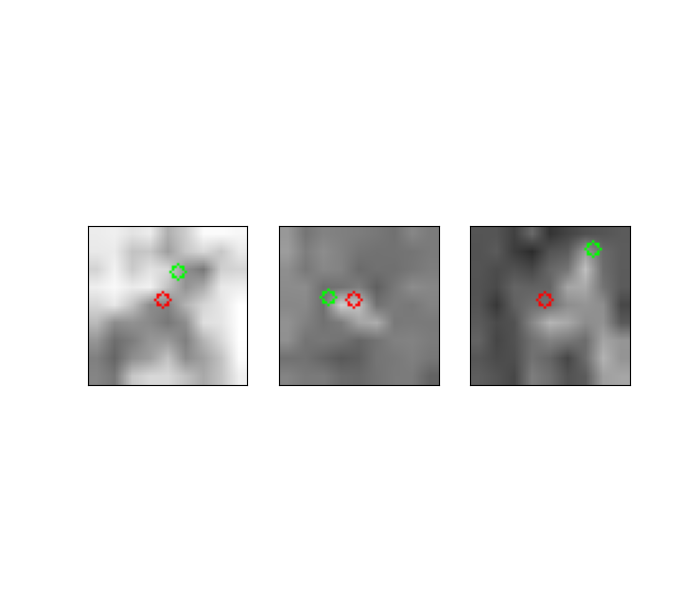
\includegraphics[width=9cm]{images/Refinado2.png}
\caption{Puntos refinados para yosemite2}
\label{fig:2figsB}
\end{minipage}
\end{figure}
\section*{Ejercicio 2: Detección de correspondencias}
Este ejercicio pide estudiar las correspondencias entre los puntos extraídos usando el descriptor KAZE. Para ello, hacemos uso de la función de OpenCV AKAZE create y extraemos los keypoints y sus descriptores con detectAndCompute:
\begin{center}
\texttt{cv2.AKAZE$\_$create().detectAndCompute(im, None)}
\end{center}
También nos pide establecer las correspondencias existentes entre las dos imágenes del punto anterior usando el objeto BFMatcher de OpenCV y los criterios de correspondencias “BruteForce+crossCheck" y “Lowe-Average-2NN”. Usamos en ambos la distancia de Hamming.\\
El primero corresponde un punto con el punto con
descriptor más cercano en la otra imagen. El parámetro crossCheck obliga a que esta correspondencia sea en ambos sentidos. Para ello he definido una función que crea el objeto pedido:
\begin{center}
\texttt{def matchesBruteforce(desc1, desc2):}\\
$\#$Creamos el objeto BFMatcher mas crossCheck\\
\texttt{bf = cv2.BFMatcher$\_$create(normType = cv2.NORM$\_$HAMMING, crossCheck = True)}\\
$\#$Calculamos los matches entre descriptores\\
\texttt{matches = bf.match(desc1, desc2)}
\end{center}
En cambio, el segundo creiterio “Lowe-Average-2NN” considera para cada descriptor los dos más cercanos en la otra imagen y elegimos uno de ellos solo si el cociente entre la distancia más cercana y la segunda más cercana debe ser menor que un cierto umbral, que fijamos a 0.75.\\
Seleccionamos ahora 100 puntos aleatorios y mediante rectas mostramos las correspondencias, como se hace en la función \texttt{getMatches}.
\begin{center}
\texttt{im$\_$matches$\_$2nn = cv2.drawMatches(im1, kp1, im2, kp2, match$\_$2nn, None,flags = cv2.DRAW$\_$MATCHES$\_$FLAGS$\_$NOT$\_$DRAW$\_$SINGLE$\_$POINTS)}\\
\texttt{im$\_$matches$\_$bf = cv2.drawMatches(im1, kp1, im2, kp2, matches$\_$bf, None,flags = cv2.DRAW$\_$MATCHES$\_$FLAGS$\_$NOT$\_$DRAW$\_$SINGLE$\_$POINTS)}
\end{center}
Las imágenes quedan:\\
\begin{figure}[H]
\centering
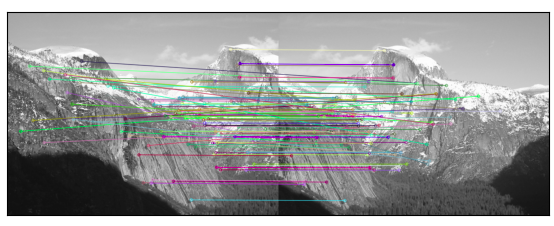
\includegraphics[scale=0.55]{images/CorrespBFCC.png} 
\caption{Correspondencias con “BruteForce+crossCheck" para Yosemite.}
\label{etiqueta}
\end{figure}
Con este primer criterio no conseguimos un resultado muy acertado, vemos a simple vista que hay varias lineas que no se corresponden bien. En cambio con el segundo, obtenemos unas correspondencias mucho más acertadas. Lo mismo pasa en las imágenes del mosaico. Esto se debe a que nos quedamos siempre con la mejor corrspondencia, estando así más seguros de que van a ser correctas.
\begin{figure}[H]
\centering
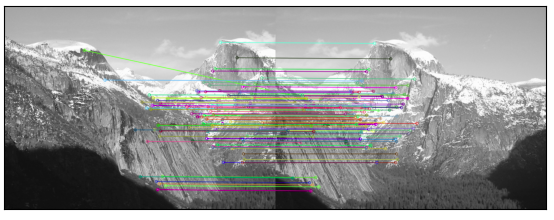
\includegraphics[scale=0.55]{images/CorrespLA2NN.png} 
\caption{Correspondencias con “Lowe-Average-2NN” para Yosemite.}
\label{etiqueta}
\end{figure}
\begin{figure}[H]
\centering
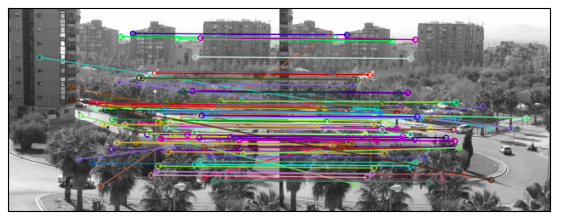
\includegraphics[scale=0.55]{images/CorrespMosaicoBFCC.png} 
\caption{Correspondencias con “BruteForce+crossCheck" para Mosaico.}
\label{etiqueta}
\end{figure}
\begin{figure}[H]
\centering
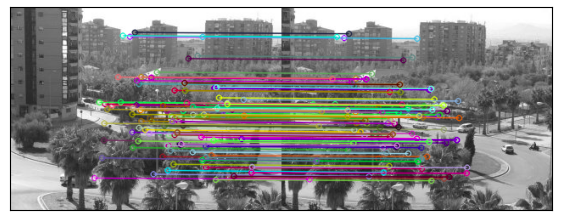
\includegraphics[scale=0.55]{images/CorrespMosaicoLA2NN.png} 
\caption{Correspondencias con “Lowe-Average-2NN” para Mosaico.}
\label{etiqueta}
\end{figure}

\section*{Ejercicio 3: Creación de un mosaico de tres imágenes}
Para este ejercicio, he probado con las dos imágenes de Yosemite, y la función que lo resuelve sólo admite dos imágenes. Si hubiera una tercera imagen solo habría pasarle la imagen resultante del mosaico y la nueva imagen a añadir, como he ejemplificado con tres imagenes de "mosaico".\\
La variable canvas es donde irá la imagen resultado. La rellenamos de ceros con la altura de las imágenes a unir y con una estimación de lo que van a medir de largo juntas e incluimos la primera imagen a la izquierda. Posteriormente, estimamos una homografía desde la segunda imagen a la primera, para después componer con la homografía de la primera imagen al mosaico (la identidad) y obtener una homografía que lleve la segunda imagen en el mosaico.\\
Para estimar la homografía usamos los descriptores y las correspondencias de la segunda imagen a la primera, que ya fueron calculados en el aprtado anterior. Una vez conseguidos, la función \texttt{findHomography} de OpenCV nos permite estimar la homografía buscada. Le decimos que use el método RANSAC para conseguir una estimación más robusta. Esto lo implemento en la función \texttt{getHomography}.\\
Por último queda trasladar la segunda imagen al mosaico. Para ello hacemos uso de la función de OpenCV \texttt{warpPerspective} que aplica la homografía. Los resultados en imágenes quedan:
\begin{figure}[H]
\centering
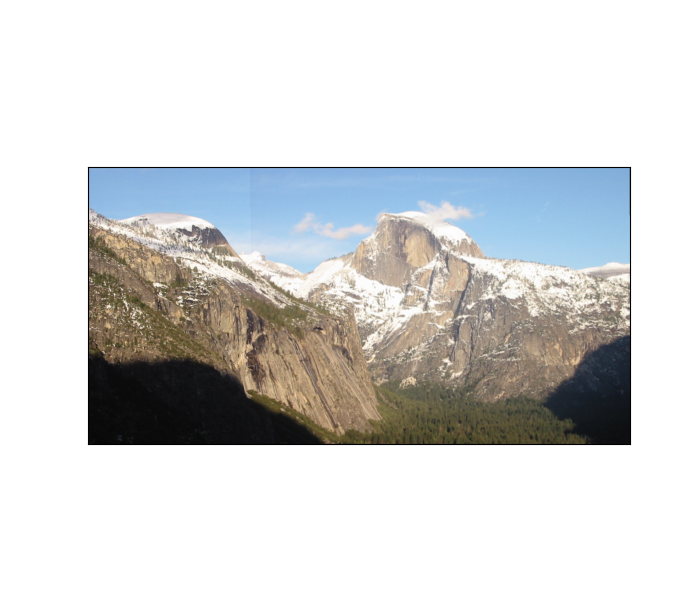
\includegraphics[scale=0.55]{images/Ejercicio3.png} 
\caption{Mosaico para las dos imagenes de Yosemite.}
\label{etiqueta}
\end{figure}
\begin{figure}[H]
\centering
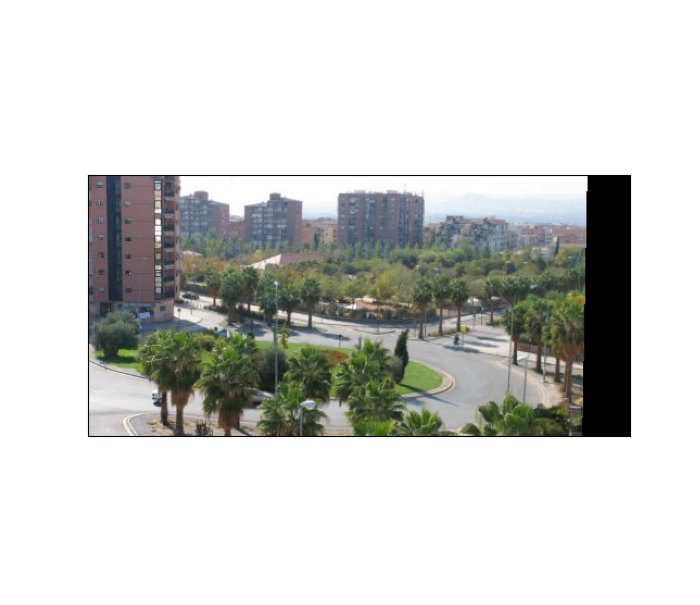
\includegraphics[scale=0.55]{images/Ejercicio3-2.png} 
\caption{Mosaico para tres imagenes consecutivas de mosaico.}
\label{etiqueta}
\end{figure}
Observamos que salvo un cambio de color en la región de solapamiento, el mosaico se obtiene de forma satisfactoria.
\section*{Ejercicio 4: Creación de un mosaico de varias imágenes}
Al igual que el ejericio anterior, tenemos que crear un mosaico pero esta vez de un número arbitrario de imágenes. Ahora lo que hacemos es ir ajustando manuelmente el canvas para que quepan todas las imágenes. Como nos dicen que se han tomado las imágenes de derecha a izquierda, podemos suponer que leyéndolas en orden habrá homografías entre las imágenes N y N-1.\\
Para crear el mosaico, ponemos la imagen central en él y vamos añadiendo a los lados según si su índice es mayor o menor que el central. Es decir, para las imágenes que están a la izquierda de la imagen central queremos estimar la homografía entre cada imagen y la siguiente y para las que están a la derecha de la imagen central queremos estimar homografías entre una imagen y la anterior. Esto lo conseguimos con el primer bucle de la función \texttt{ejercicio4}. Para añadir las imágenes al mosaico aprovechamos que lo tenemos hecho para parejas de imágenes, así que las vamos recorriendo comenzando por las que rodean a la central y avanzando hacia los extremos.\\
Por último, calculamos todo esto para cada imagen de "mosaico", dando como resultado la siguiente panorámica:\\
\begin{figure}[H]
\centering
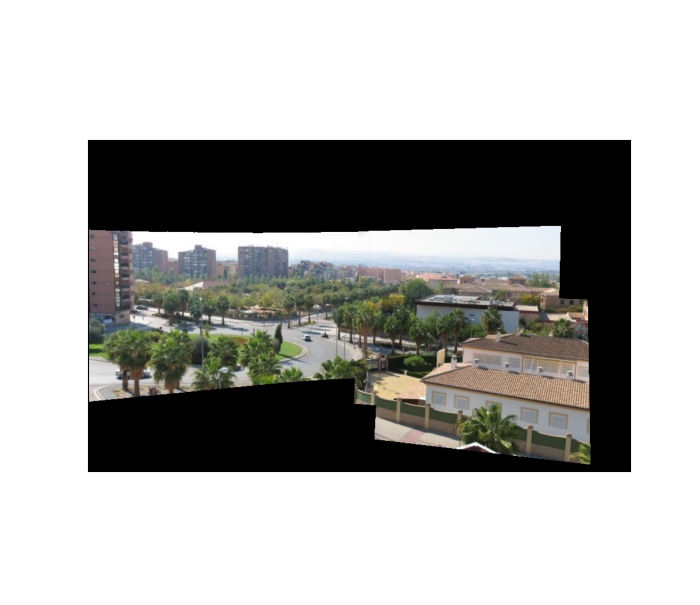
\includegraphics[scale=0.55]{images/Ejercicio4.png} 
\caption{Mosaico para las imagenes consecutivas de "mosaico".}
\label{etiqueta}
\end{figure}
Donde podemos observar que el solapamiento es satisfactorio a pesar de que la imagen final no es rectangular. Esto es debido a la forma en la que se tomó la foto (desde un solo punto y de forma circular) y a errores de cálculo de los descriptores.


% --------------------------------------------------------------
%     You don't have to mess with anything below this line.
% --------------------------------------------------------------
 
\end{document}